 \chapter{Experimentos y Resultados} 
En la siguiente sección, se demuestra el funcionamiento de los objetivos generales y 
propuestos en la sección \ref{cap:objGeneral} y \ref{cap:objEspec} respectivamente.

\section{Pruebas de la mesa de servicio, como servicio web.}
Como ya lo hemos visto en capítulos anteriores, un servicio web es una tecnología que permite la comunicación y el intercambio de información entre diferentes aplicaciones y sistemas a través de Internet.

Por lo anterior nuestro sistema, cumple con dicho requerimiento derivado, de su arquitectura web tanto en backend, como en el frontend.

Para demostración se tomara como ecenario  de prueba, el inicio de sesión, como se muestra en la figura \ref{fig:lognas}	

 \begin{figure}[H]
	\centering
	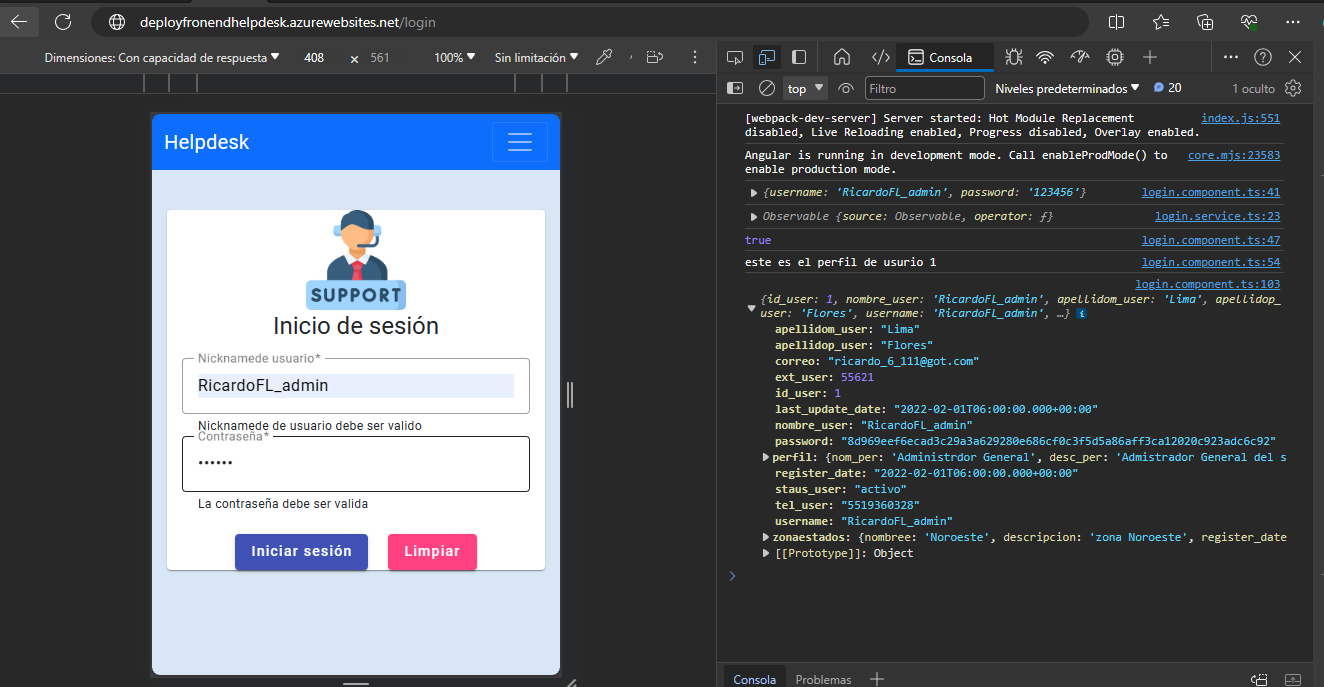
\includegraphics[width=0.9\textwidth]{Capitulo7/Img/login}
	\caption{Login de Helpdesk}
	\label{fig:lognas}
\end{figure}
\section{Pruebas del Flujo de Trabajo según ITIL}
ITIL como parte de su marco de trabajo solicta que se organice a los colabores, por roles o activases a desarrollar,  para su eficiente  gestión los servicios de TI que se ofrecen a un cliente, por lo cual, el sistema  Mesa de Servicio  cuenta con un panel de administración de usuarios como se muestra en la figura \ref{fig:user}
 \begin{figure}[H]
	\centering
	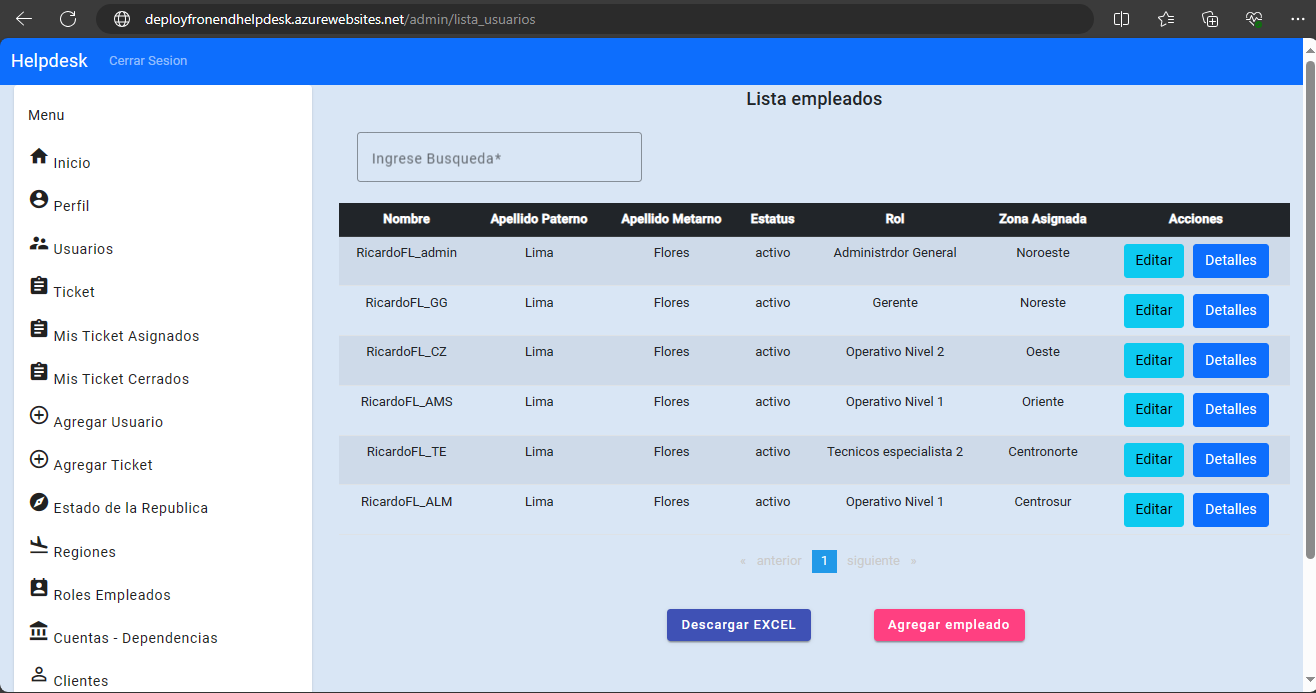
\includegraphics[width=1.1\textwidth]{Capitulo7/Img/usuarios}
	\caption{Administración de Usuarios}
	\label{fig:user}
\end{figure}

\subsection{Fundamentos de ITIL - Gestión de incidencias}

Gestionar las incidencias de forma proactiva utilizando ITIL hace que haya menos incidencias repetitivas y también graves. La automatización ayuda a la clasificación y asignación de los tickets de asistencia, de manera que los agentes del Service Desk puedan centrarse las incidencias prioritarias.

Por lo anterior, de describirá el ciclo de vida de un Ticket:

\begin{enumerate}
	\item  \textbf{Creación de Ticket}:
	En la figura \ref{fig:ticketdrw} se muestra el formulario el cual deberá ser llenado con la información, como lo es la descripcion del error, numero de Serie del equipo a atender, nombre del cliente quien solicita el servicio, entidad federativa donde se estará atendiendo, servicio que se estará dando y estatus del ticket.
	 \begin{figure}[H]
		\centering
		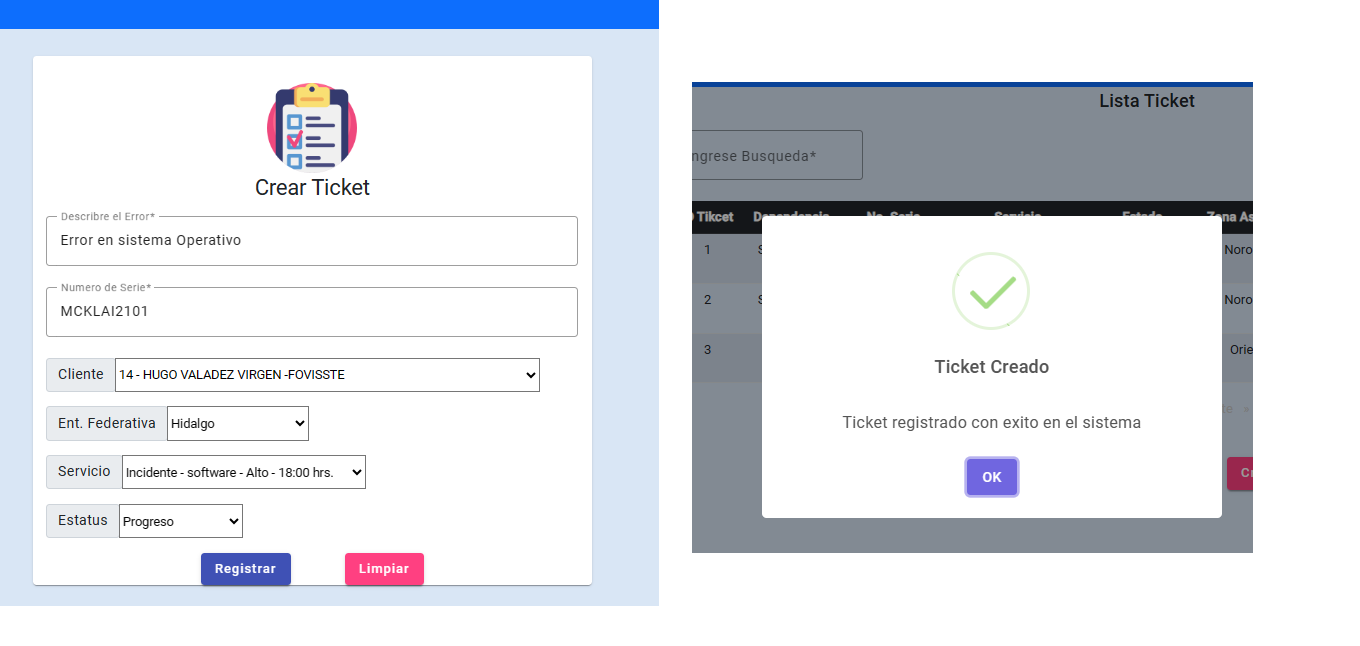
\includegraphics[width=1.1\textwidth]{Capitulo7/Img/creaticket}
		\caption{Registro de Ticket en el sistema}
		\label{fig:ticketdrw}
	\end{figure}
\item  \textbf{Incorporación a la Lista de Ticket en proceso de atención}:
	En la figura \ref{fig:ListaTicket} se muestra el ticket creado, así como datos relevantes del mismo,  de igual forma las acciones que se pueden tomar como, \textbf{Asignar, Editar y Documentar}
	
	\begin{figure}[H]
		\centering
		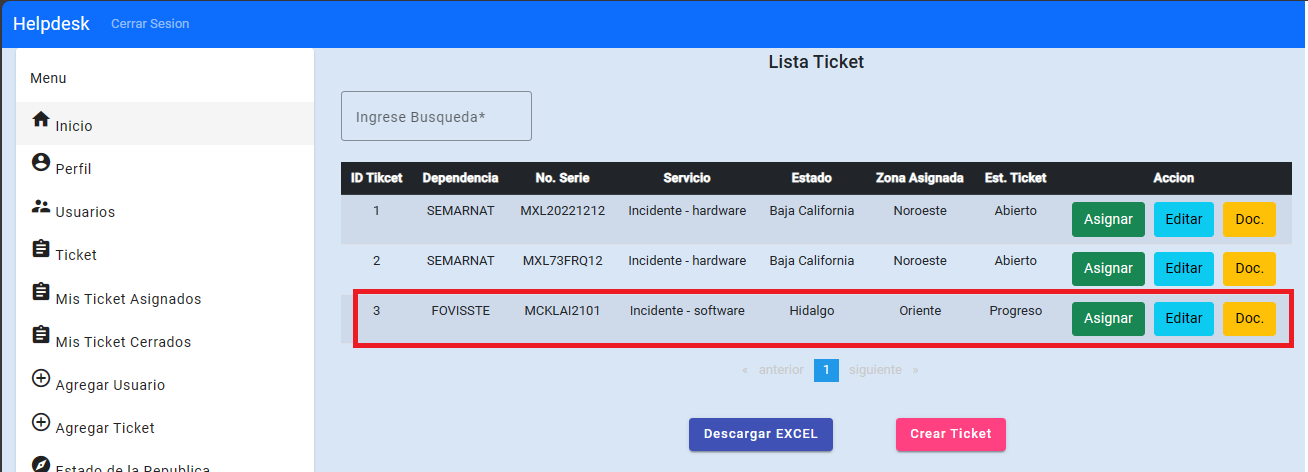
\includegraphics[width=1.1\textwidth]{Capitulo7/Img/ListaTicket}
		\caption{Lista de Ticket Creados}
		\label{fig:ListaTicket}
	\end{figure}



\item  \textbf{Asignacion de Ticket a Colaborador}:
En la figura \ref{fig:asignacion} se muestra el formulario el cual deberá ser llenado con la información, como lo es una breve descripcion de la asignacion, así como la selección del colaborador al cual le sera asignada la atención. 

\begin{figure}[H]
	\centering
	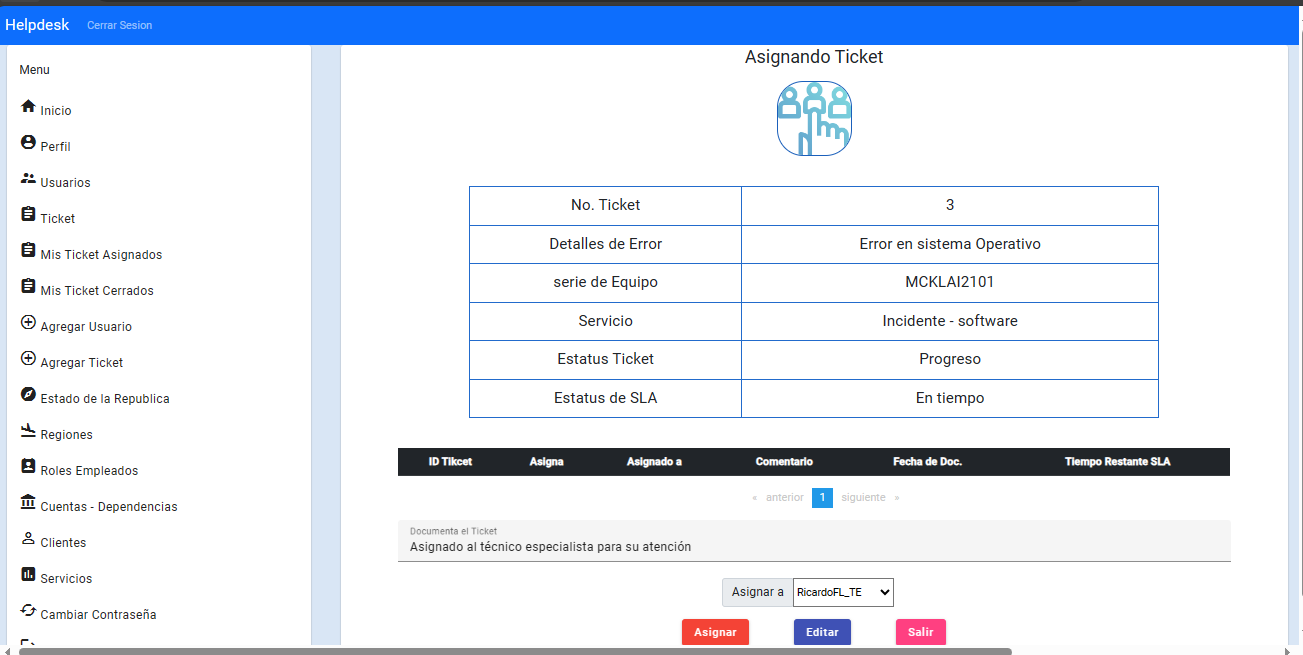
\includegraphics[width=1.1\textwidth]{Capitulo7/Img/asignacion}
	\caption{Asignacion de Ticket}
	\label{fig:asignacion}
\end{figure}
	
	\item  \textbf{Documentación de Ticket}:
	En la figura \ref{fig:doc} se muestra el formulario el cual deberá ser llenado con la información del proceso del ticket, cabe mencionar que este sera el historial de atención del Ticket. 
	
	\begin{figure}[H]
		\centering
		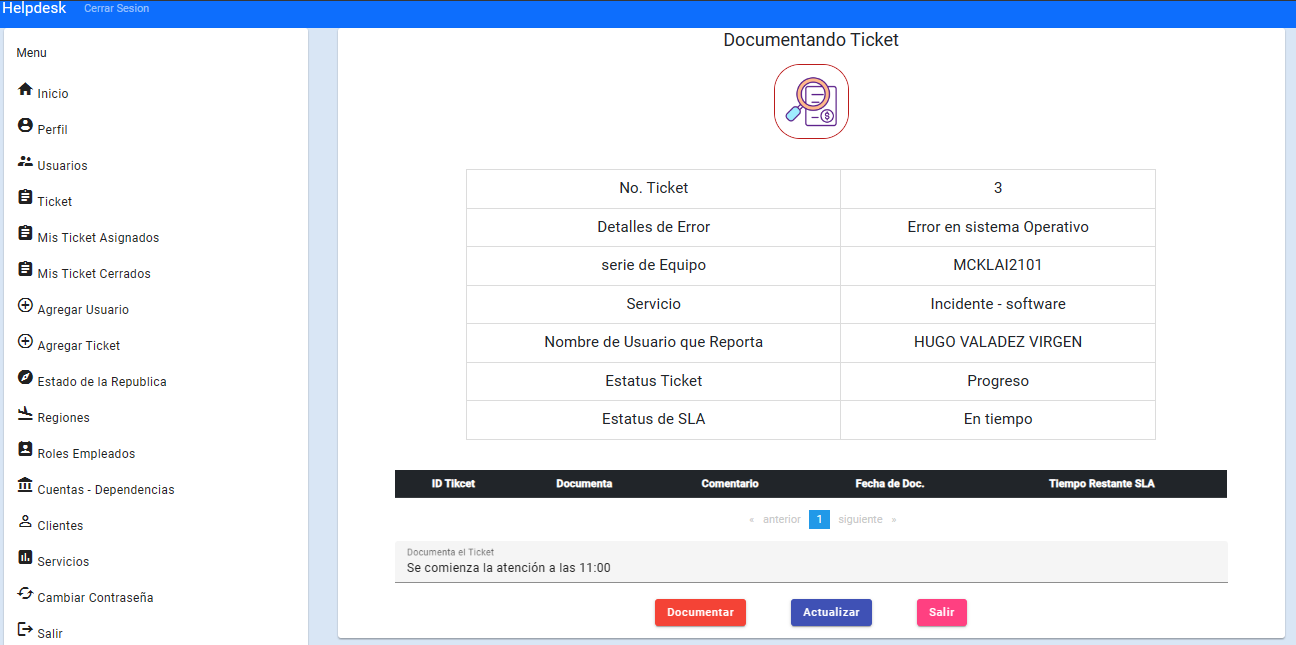
\includegraphics[width=1.1\textwidth]{Capitulo7/Img/doc}
		\caption{Documentación de Ticket}
		\label{fig:doc}
	\end{figure}


	\item  \textbf{Documentación de Ticket}:
En la figura \ref{fig:cierre} se muestra el formulario el cual deberá ser modificado, tal modificación unicamente debe de realizare en el Estatus del ticket cambiando a cerrado. 

\begin{figure}[H]
	\centering
	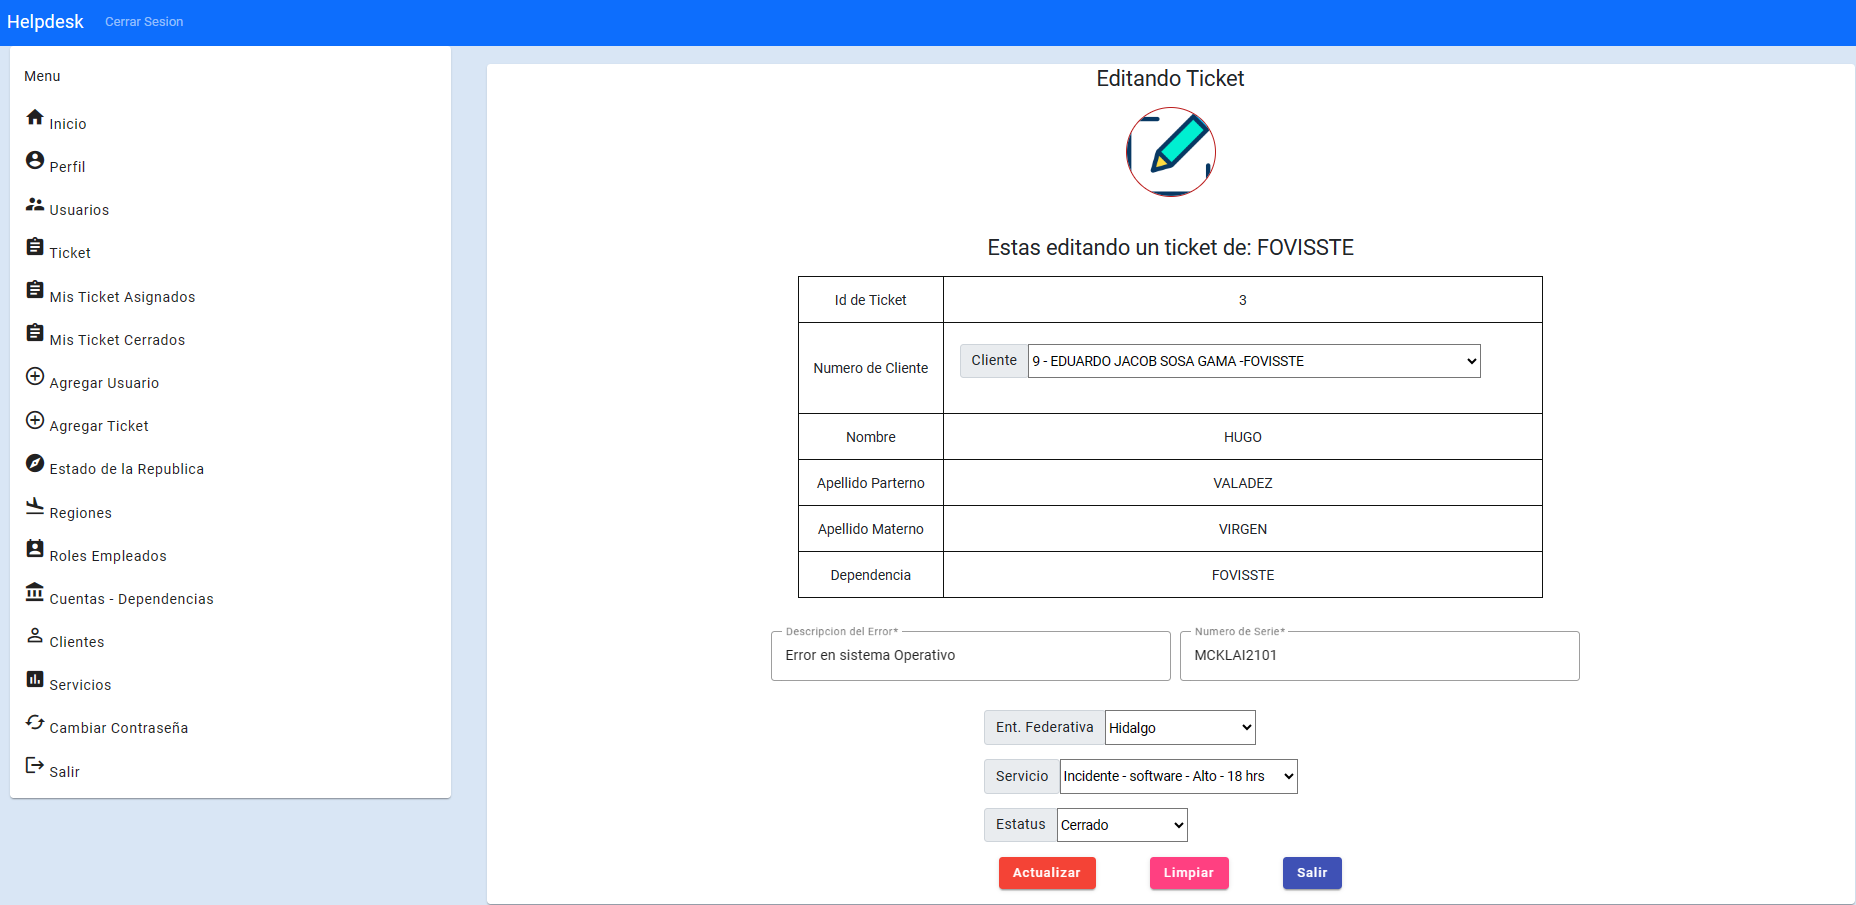
\includegraphics[width=1.1\textwidth]{Capitulo7/Img/cierre}
	\caption{Cierre de Ticket}
	\label{fig:cierre}
\end{figure}

	
\end{enumerate}